\section{Aplicación propuesta}

% Arquitectura General
\begin{frame}{Arquitectura General}
  \begin{figure}
    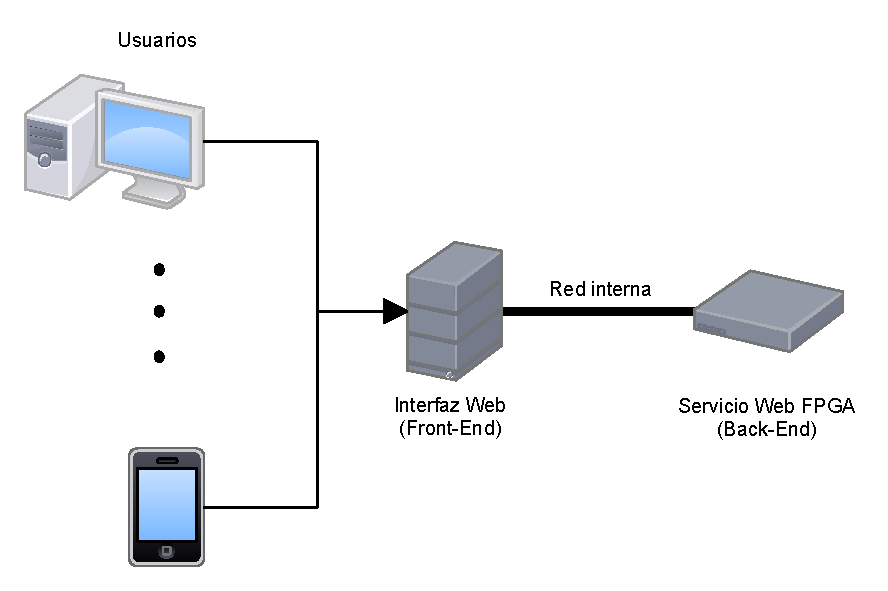
\includegraphics[width=0.9\linewidth]{arquitectura}
  \end{figure}
\end{frame}

% Stack de tecnologías
\begin{frame}{Stack tecnológico}
  \begin{itemize}
    \item\alert<+>{Back-End}
    \begin{itemize}
      \item JavaScript
      \item node.js
      \item express, async, nodemon
    \end{itemize}
    \item\alert<+>{Front-End}
    \begin{itemize}
      \item PHP (HTML, JavaScript, CSS)
      \item Framework propio
      \item Bootstrap, jQuery
    \end{itemize}
  \end{itemize}
\end{frame}

% Back-End
\begin{frame}{Back-End - Servicio Web FPGA}
  \begin{itemize}[<alert@+>]
    \item Formalizar y exponer la funcionalidad de la FPGA
    \item Permite conocer el estado de la misma y de aspectos relacionados
    \item Implementación REST-like
  \end{itemize}
  \begin{figure}
    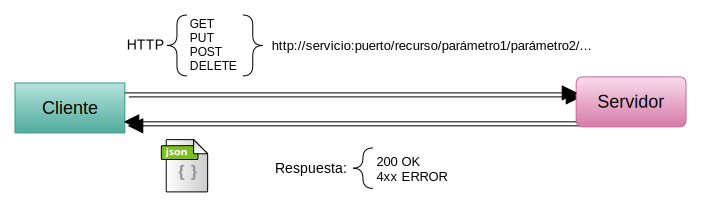
\includegraphics[width=\linewidth]{fpga_rest}
  \end{figure}
\end{frame}

\begin{frame}{Back-End - Arquitectura interna}
  \begin{figure}
    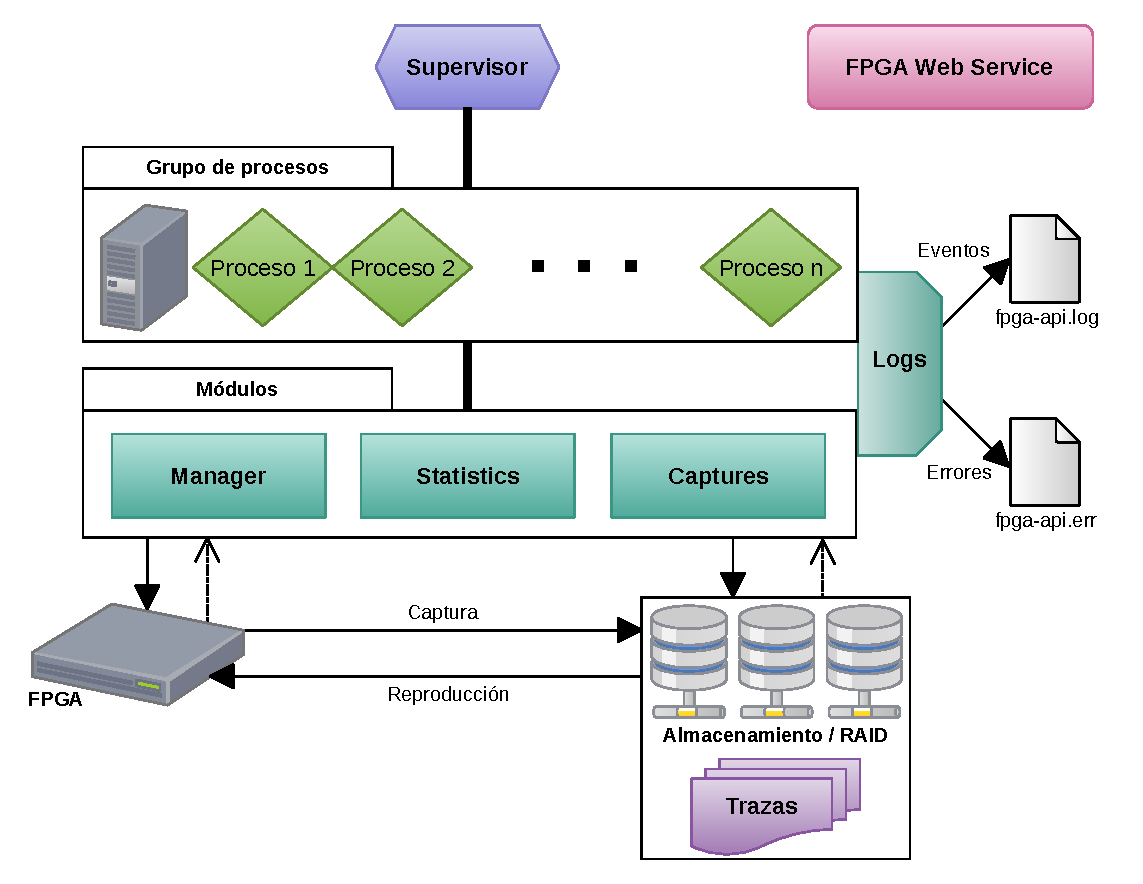
\includegraphics[width=0.85\linewidth]{fpga}
  \end{figure}
\end{frame}

\begin{frame}{Back-End - FSM Estado FPGA}
  \begin{figure}
    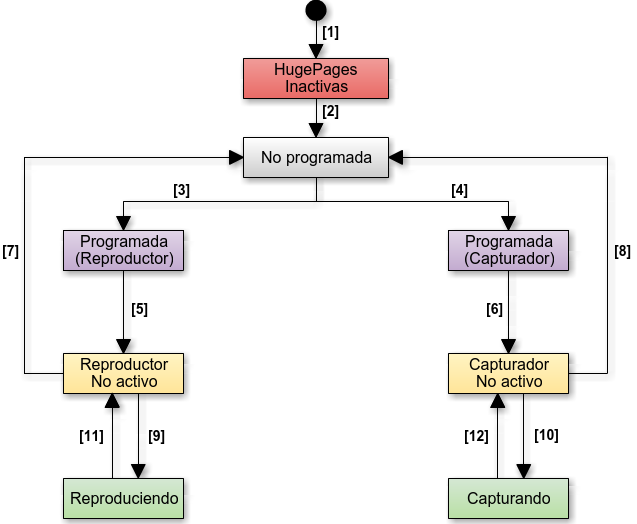
\includegraphics[width=0.65\linewidth, valign=t]{fpga_estado}
    \hfill
    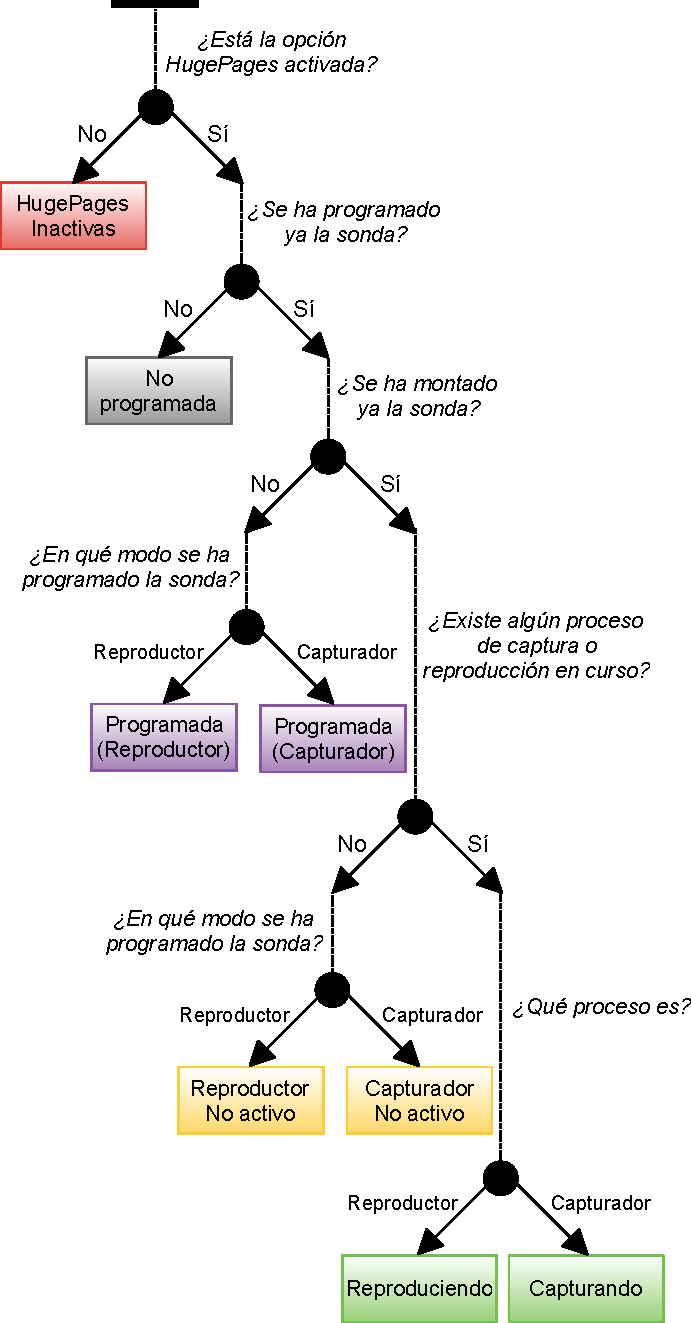
\includegraphics[height=0.7\textheight, valign=t]{arbol_decision_vertical}
  \end{figure}
\end{frame}

\begin{frame}{Back-End - API REST}
  \begin{figure}
    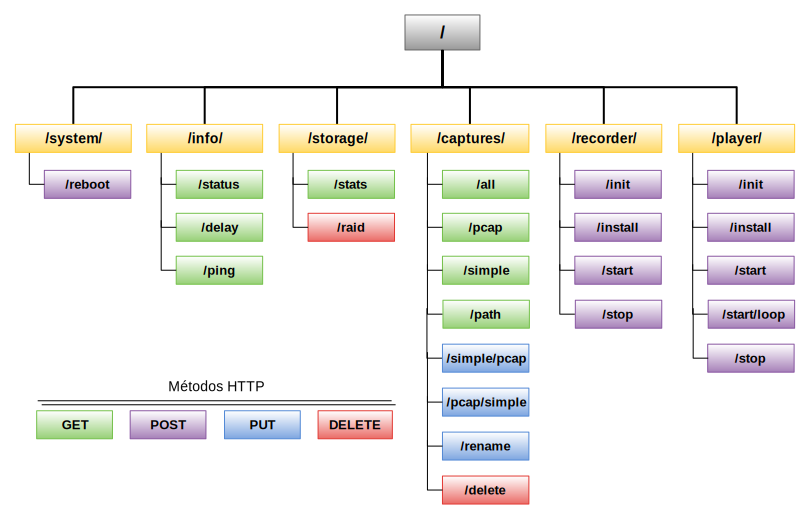
\includegraphics[width=\linewidth]{arbol_metodos}
  \end{figure}
\end{frame}

% Front-End
\begin{frame}{Front-End}
  \begin{itemize}[<alert@+>]
    \item Comunicación con el back-end (proxy)
    \item Framework propio
    \item Diseño \textit{responsive}
  \end{itemize}
\end{frame}

\begin{frame}{Front-End - Framework - Arquitectura interna}
  \begin{figure}
    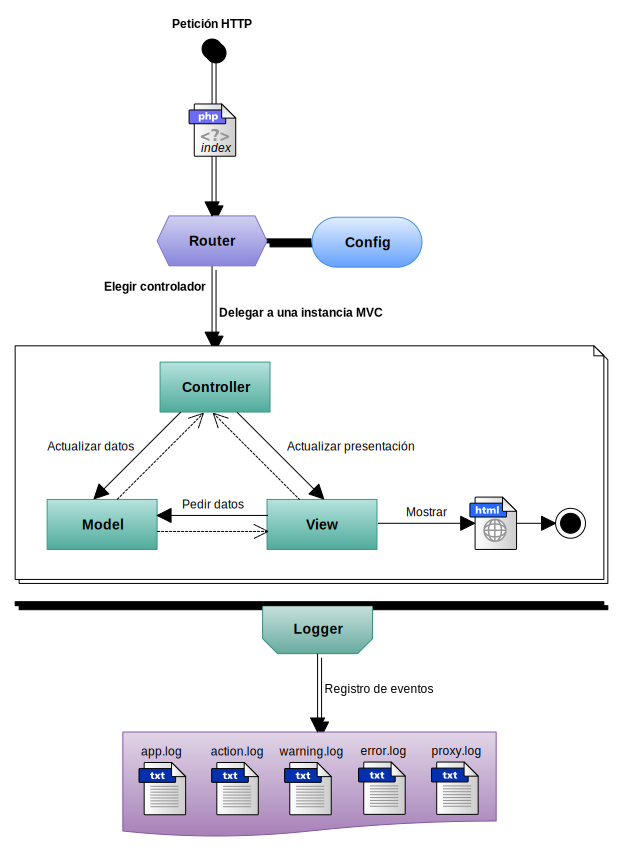
\includegraphics[width=\linewidth]{framework}
  \end{figure}
\end{frame}

\begin{frame}{Front-End - Framework - Router}
  \begin{figure}
    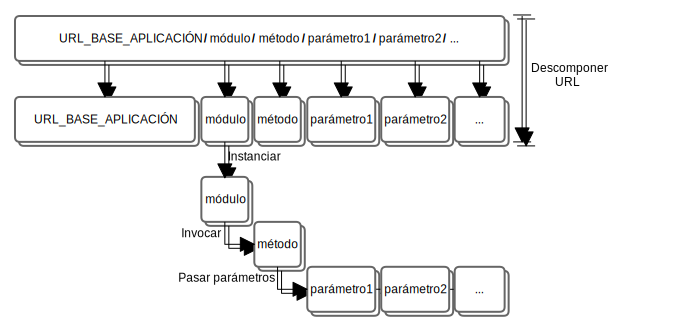
\includegraphics[width=\linewidth]{router}
  \end{figure}
\end{frame}

\begin{frame}{Front-End - Framework - Proxy}
  \begin{figure}
    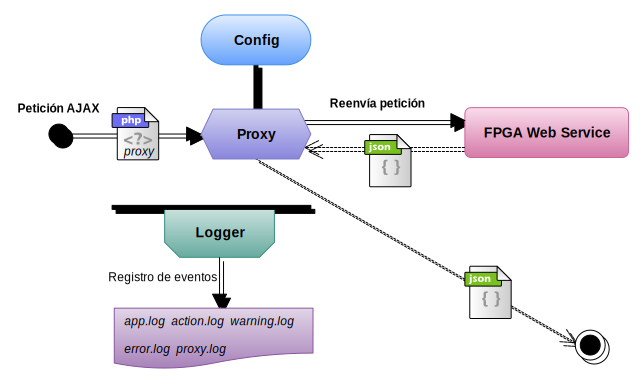
\includegraphics[width=\linewidth]{proxy}
  \end{figure}
\end{frame}

\begin{frame}{Front-End - Diseño - Capturas}
  \begin{figure}
    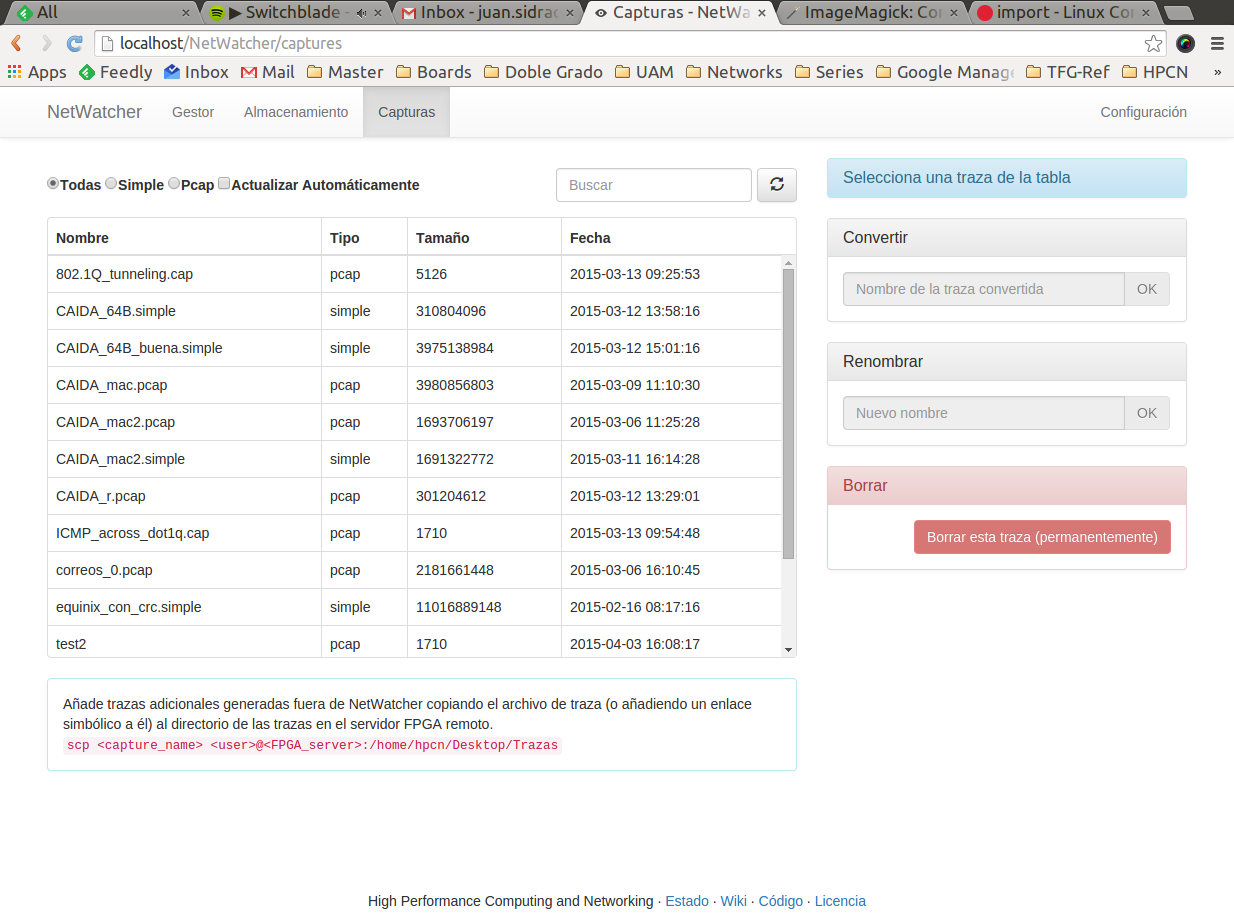
\includegraphics[width=\linewidth]{capturas}
  \end{figure}
\end{frame}

\begin{frame}{Front-End - Diseño - Gestor capturar}
  \begin{figure}
    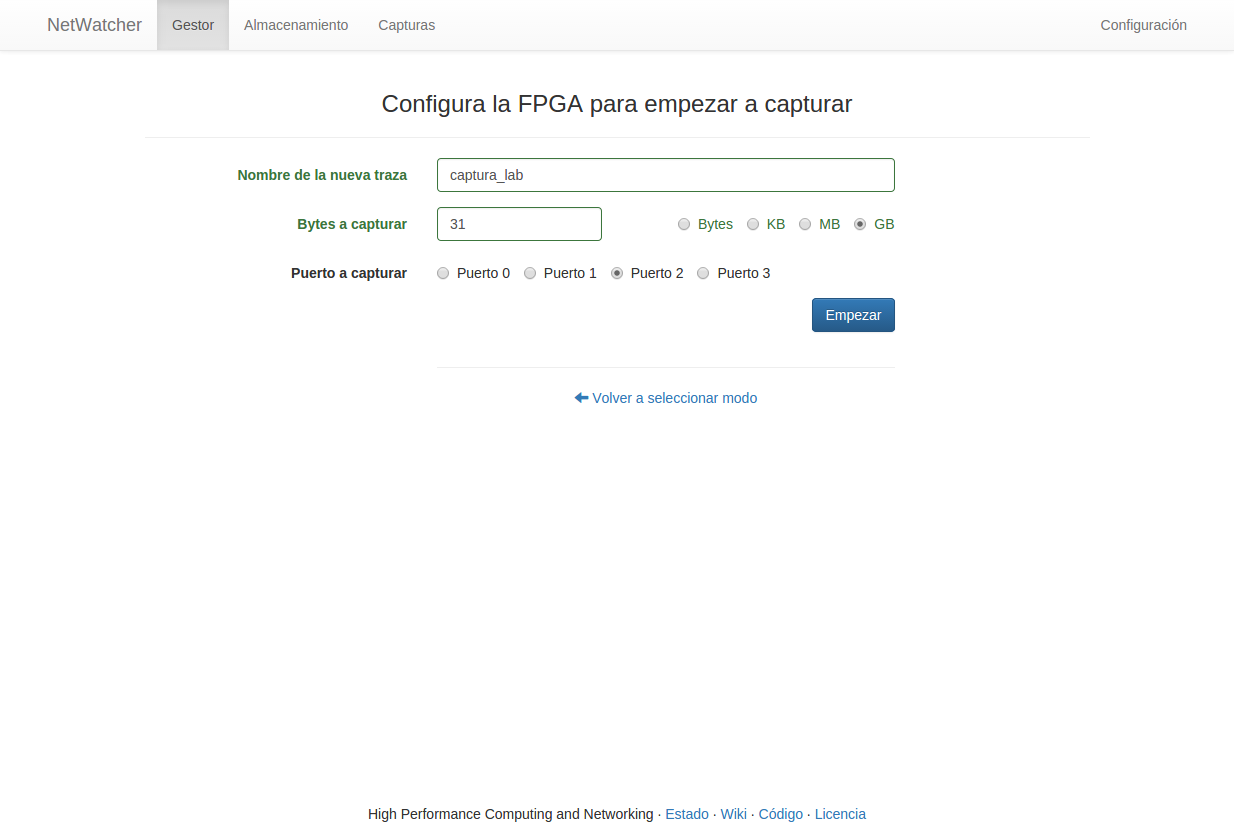
\includegraphics[width=\linewidth]{gestor_capturar}
  \end{figure}
\end{frame}

\begin{frame}{Front-End - Diseño - Estado}
  \begin{figure}
    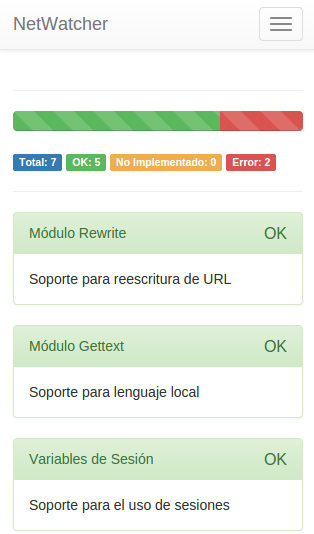
\includegraphics[width=0.3\linewidth]{estado_movil}
  \end{figure}
\end{frame}
